%%% Title:    IDS Lecture 4
%%% Author:   Kyle M. Lang
%%% Created:  2017-09-12
%%% Modified: 2020-04-20

\documentclass{beamer}\usepackage[]{graphicx}\usepackage[]{color}
% maxwidth is the original width if it is less than linewidth
% otherwise use linewidth (to make sure the graphics do not exceed the margin)
\makeatletter
\def\maxwidth{ %
  \ifdim\Gin@nat@width>\linewidth
    \linewidth
  \else
    \Gin@nat@width
  \fi
}
\makeatother

\definecolor{fgcolor}{rgb}{0, 0, 0}
\newcommand{\hlnum}[1]{\textcolor[rgb]{0.69,0.494,0}{#1}}%
\newcommand{\hlstr}[1]{\textcolor[rgb]{0.749,0.012,0.012}{#1}}%
\newcommand{\hlcom}[1]{\textcolor[rgb]{0.514,0.506,0.514}{\textit{#1}}}%
\newcommand{\hlopt}[1]{\textcolor[rgb]{0,0,0}{#1}}%
\newcommand{\hlstd}[1]{\textcolor[rgb]{0,0,0}{#1}}%
\newcommand{\hlkwa}[1]{\textcolor[rgb]{0,0,0}{\textbf{#1}}}%
\newcommand{\hlkwb}[1]{\textcolor[rgb]{0,0.341,0.682}{#1}}%
\newcommand{\hlkwc}[1]{\textcolor[rgb]{0,0,0}{\textbf{#1}}}%
\newcommand{\hlkwd}[1]{\textcolor[rgb]{0.004,0.004,0.506}{#1}}%
\let\hlipl\hlkwb

\usepackage{framed}
\makeatletter
\newenvironment{kframe}{%
 \def\at@end@of@kframe{}%
 \ifinner\ifhmode%
  \def\at@end@of@kframe{\end{minipage}}%
  \begin{minipage}{\columnwidth}%
 \fi\fi%
 \def\FrameCommand##1{\hskip\@totalleftmargin \hskip-\fboxsep
 \colorbox{shadecolor}{##1}\hskip-\fboxsep
     % There is no \\@totalrightmargin, so:
     \hskip-\linewidth \hskip-\@totalleftmargin \hskip\columnwidth}%
 \MakeFramed {\advance\hsize-\width
   \@totalleftmargin\z@ \linewidth\hsize
   \@setminipage}}%
 {\par\unskip\endMakeFramed%
 \at@end@of@kframe}
\makeatother

\definecolor{shadecolor}{rgb}{.97, .97, .97}
\definecolor{messagecolor}{rgb}{0, 0, 0}
\definecolor{warningcolor}{rgb}{1, 0, 1}
\definecolor{errorcolor}{rgb}{1, 0, 0}
\newenvironment{knitrout}{}{} % an empty environment to be redefined in TeX

\usepackage{alltt}
\usetheme[%
  pageofpages          = of,
  bullet               = circle,
  titleline            = true,
  alternativetitlepage = true,
  titlepagelogo        = Logo3,
  watermark            = watermarkTiU,
  watermarkheight      = 100px,
  watermarkheightmult  = 4%
]{UVT}

\usepackage{graphicx}
\usepackage[natbibapa]{apacite}
\usepackage[libertine]{newtxmath}
\usepackage{booktabs}
\usepackage{fancybox}

\newcommand{\kfold}[0]{\emph{K}-fold cross-validation}

%% Ensure styles of `blocks' (used in Definitions, Theorems etc.) follows the
%% UVT-style theme:
\setbeamercolor{block title}{fg = darkblue, bg = white}
\setbeamercolor{block body}{use = block title, bg = block title.bg}

%% Ensure TableOfContents is in UVT-style theme:
\setbeamercolor{section in toc}{fg = darkblue}

\title{The Generalized Linear Model \& Logistic Regression}
\subtitle{Introduction to Data Science Lecture 4}
\author{Kyle M. Lang}
\institute{Department of Methodology \& Statistics\\Tilburg University}
\date{Block 4 2020}
\IfFileExists{upquote.sty}{\usepackage{upquote}}{}
\begin{document}



%------------------------------------------------------------------------------%

\begin{frame}[t,plain]
\titlepage
\end{frame}

%------------------------------------------------------------------------------%

\begin{frame}{Outline}
  
  \begin{enumerate}
  \item Generalized linear models
    \vb
  \item Logistic regression
    \vb
  \item Multinomial logistic regression
    \vb
  \item Classification via logistic regression
  \end{enumerate}
  
\end{frame}

%------------------------------------------------------------------------------%

\begin{frame}{General Linear Model}
  
  So far, we've been discussing models with this form:
  \begin{align*}
    Y = \beta_0 + \sum_{p = 1}^P \beta_p X_p + \varepsilon
  \end{align*}
  This type of model is known as the \emph{general linear model}.
  \vc
  \begin{itemize}
  \item All flavors of linear regression are general linear models.
    \vc
    \begin{itemize}
    \item ANOVA
    \item ANCOVA
    \item Multilevel linear regression models
    \end{itemize}
  \end{itemize}
  
\end{frame}

%------------------------------------------------------------------------------%

\begin{frame}{Components of the General Linear Model}
 
  We can break our model into pieces:
  \begin{align*}
    \eta &= \beta_0 + \sum_{p = 1}^P \beta_p X_p\\
    Y &= \eta + \varepsilon
  \end{align*}
  Because $\varepsilon \sim \text{N}(0, \sigma^2)$, we can also write:
  \begin{align*}
    Y \sim \text{N}(\eta, \sigma^2)
  \end{align*}
  In this representation:
  \begin{itemize}
  \item $\eta$ is the \emph{systematic component} of the model
  \item The normal distribution, $\text{N}(\cdot, \cdot)$, is the model's 
    \emph{random component}.
  \end{itemize}
  
\end{frame}

%------------------------------------------------------------------------------%

\begin{frame}{Components of the General Linear Model}
  
  The purpose of general linear modeling (i.e., regression modeling) is to build
  a model of the outcome's mean, $\mu_Y$.  
  \begin{itemize}
  \item In this case, $\mu_Y = \eta$.
  \item The systematic component defines the mean of $Y$.
  \end{itemize}
  \vb
  The random component quantifies variability (i.e., error variance) around
  $\mu_Y$.  
  \begin{itemize}
  \item In the general linear model, we assume that this error variance follows
    a normal distribution.
  \item Hence the normal random component.
  \end{itemize}
  
\end{frame}

%------------------------------------------------------------------------------%

\begin{frame}{Generalized Linear Model}
  
  We can generalize the models we've been using in two important ways:
  \vc
  \begin{enumerate}
  \item Allow for random components other than the normal distribution.
    \vc
  \item Allow for more complicated relations between $\mu_Y$ and $\eta$.
    \begin{itemize}
    \item Allow: $g(\mu_Y) = \eta$
    \end{itemize}
  \end{enumerate}
  \vc
  These extensions lead to the class of \emph{generalized linear models} (GLMs).
  
\end{frame}

%------------------------------------------------------------------------------%

\begin{frame}{Components of the Generalized Linear Model}
  
  The random component in a GLM can be any distribution from the so-called 
  \emph{exponential family}.
  \vc
  \begin{itemize}
  \item The exponential family contains many popular distributions:
    \vc
    \begin{itemize}
    \item Normal
    \item Binomial
    \item Poisson
    \item Many others...
    \end{itemize}
  \end{itemize}
  \vc
  The systematic component of a GLM is exactly the same as it is in general 
  linear models:
  \begin{align*}
    \eta = \beta_0 + \sum_{p = 1}^P \beta_p X_p
  \end{align*}
  
\end{frame}

%------------------------------------------------------------------------------%

\begin{frame}{Link Functions}
  
  In GLMs, $\eta$ does not directly describe $\mu_Y$.
  \begin{itemize}
  \item We first transform $\mu_Y$ via a \emph{link function}.
  \item $g(\mu_Y) = \eta$
  \end{itemize}
  \vb
  The link function allows GLMs for outcomes with restricted ranges without 
  requiring any restrictions on the range of the $\{X_p\}$.
  \vc
  \begin{itemize}
  \item For strictly positive $Y$, we can use a \emph{log link}: 
    \begin{align*}
      \ln(\mu_y) = \eta.
    \end{align*}
  \item The general linear model employs the \emph{identity link}: 
    \begin{align*}
      \mu_y = \eta.
    \end{align*}
  \end{itemize}
  
\end{frame}

%------------------------------------------------------------------------------%

\begin{frame}{Components of the Generalized Linear Model}
  
  Every GLM is built from three components:
  \vb
  \begin{enumerate}
  \item The systematic component, $\eta$.
    \begin{itemize}
    \item A linear function of the predictors, $\{X_p\}$.
    \item Describes the association between $\mathbf{X}$ and $Y$.
    \end{itemize}
    \vb
  \item The link function, $g(\mu_Y)$.
    \begin{itemize}
    \item Transforms $\mu_Y$ so that it can take any value on the real line.
    \end{itemize}
    \vb
  \item The random component, $P(Y|g^{-1}(\eta))$
    \begin{itemize}
    \item The distribution of the observed $Y$.
    \item Quantifies the error variance around $\eta$.
    \end{itemize}
  \end{enumerate}
  
\end{frame}

%------------------------------------------------------------------------------%

\begin{frame}{General Linear Model $\subset$ Generalized Linear Model}
  
  The general linear model is a special case of GLM.
  \vb  
  \begin{enumerate}
  \item Systematic component:
    \begin{align*}
      \eta = \beta_0 + \sum_{p = 1}^P \beta_p X_p
    \end{align*}
  \item Link function:
    \begin{align*}
      \mu_Y = \eta
    \end{align*}
  \item Random component:
    \begin{align*}
      Y \sim \text{N}(\eta, \sigma^2)
    \end{align*}
  \end{enumerate}
  
\end{frame}

%------------------------------------------------------------------------------%

\begin{frame}{}
  
  \begin{center}
    \Huge{\textsc{Logistic Regression}}
  \end{center}
  
\end{frame}

%------------------------------------------------------------------------------%

\begin{frame}{Logistic Regression}
  
  So why do we care about the GLM when linear regression models have worked
  thus far?  
  \begin{itemize}
  \item In a word: Classification.
  \end{itemize}
  \vb
  In the classification task, we have a discrete, qualitative outcome.
  \begin{itemize}
  \item We will begin with the situation of two-level outcomes.
    \begin{itemize}
    \item Alive or Dead
    \item Pass or Fail
    \item Pay or Default
    \end{itemize}
  \end{itemize}
  \vb
  We want to build a model that predicts class membership based on some set of 
  interesting features.
  \begin{itemize}
  \item To do so, we will use a very useful type of GLM: \emph{logistic 
    regression}.
  \end{itemize}
  
\end{frame}

\watermarkoff %----------------------------------------------------------------%

\begin{frame}{Classification Example}

  \begin{columns}
    \begin{column}{0.5\textwidth}
      
      Suppose we want to know the effect of study time on the probability of
      passing an exam.  
      \vc
      \begin{itemize}
      \item The probability of passing must be between 0 and 1.
        \vc
      \item We care about the probability of passing, but we only observe 
        absolute success or failure.
        \vc
        \begin{itemize}
        \item $Y \in \{1, 0\}$
        \end{itemize}
      \end{itemize}
      
      \end{column}
    
    \begin{column}{0.5\textwidth}
      
\begin{knitrout}\footnotesize
\definecolor{shadecolor}{rgb}{0.878, 0.918, 0.933}\color{fgcolor}

{\centering 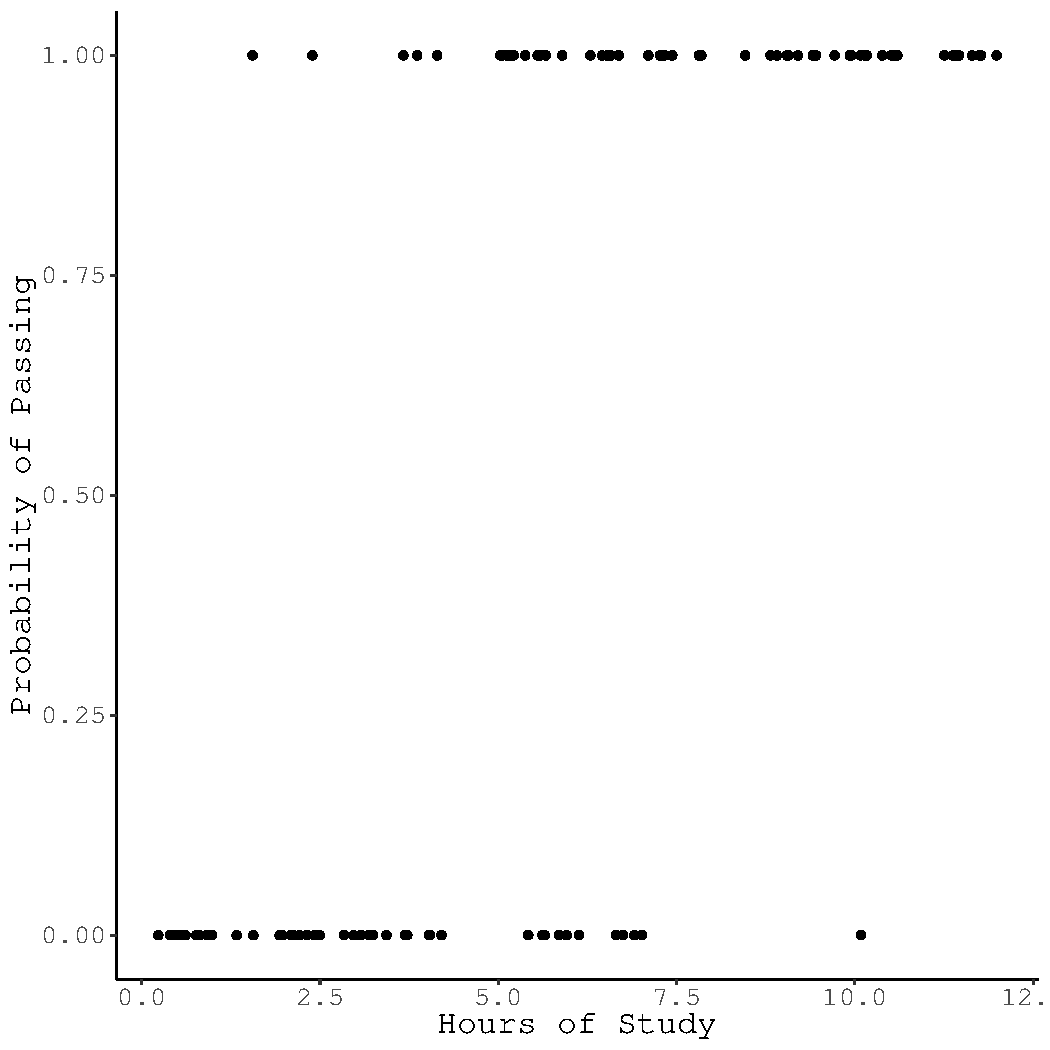
\includegraphics[width=\maxwidth]{figure/unnamed-chunk-1-1} 

}



\end{knitrout}

\end{column}
\end{columns}

\end{frame}

%------------------------------------------------------------------------------%

\begin{frame}{Linear Regression for Binary Outcomes?}

  \begin{columns}
    \begin{column}{0.5\textwidth}
      
      What happens if we try to model these data with linear regression?  
      \vc
      \begin{itemize}
      \item Hmm...notice any problems?
      \end{itemize}
      
    \end{column}
    
    \begin{column}{0.5\textwidth}
      
\begin{knitrout}\footnotesize
\definecolor{shadecolor}{rgb}{0.878, 0.918, 0.933}\color{fgcolor}

{\centering 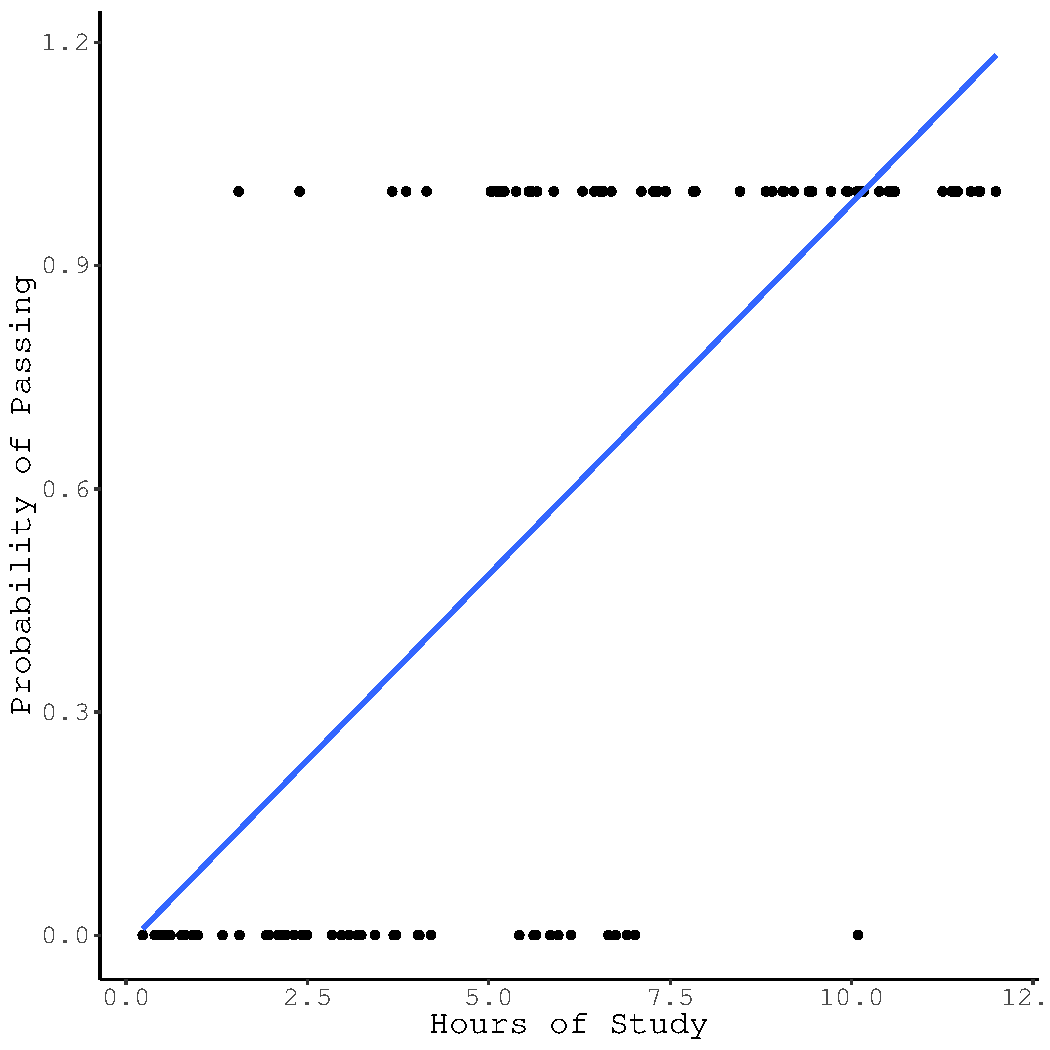
\includegraphics[width=\maxwidth]{figure/unnamed-chunk-2-1} 

}



\end{knitrout}

\end{column}
\end{columns}

\end{frame}

%------------------------------------------------------------------------------%

\begin{frame}{Logistic Regression Visualized}

  \begin{columns}
    \begin{column}{0.5\textwidth}
      
      We get a much better model using logistic regression.
      \vc
      \begin{itemize}
      \item The link function ensures legal predicted values.
        \vc
      \item The sigmoidal curve implies fluctuation in the effectiveness of
        extra study time.  
        \vc
        \begin{itemize}
        \item More study time is most beneficial for students with around 
          5.5 hours of study. 
        \end{itemize}
      \end{itemize}
      
    \end{column}
    
    \begin{column}{0.5\textwidth}
      
\begin{knitrout}\footnotesize
\definecolor{shadecolor}{rgb}{0.878, 0.918, 0.933}\color{fgcolor}

{\centering 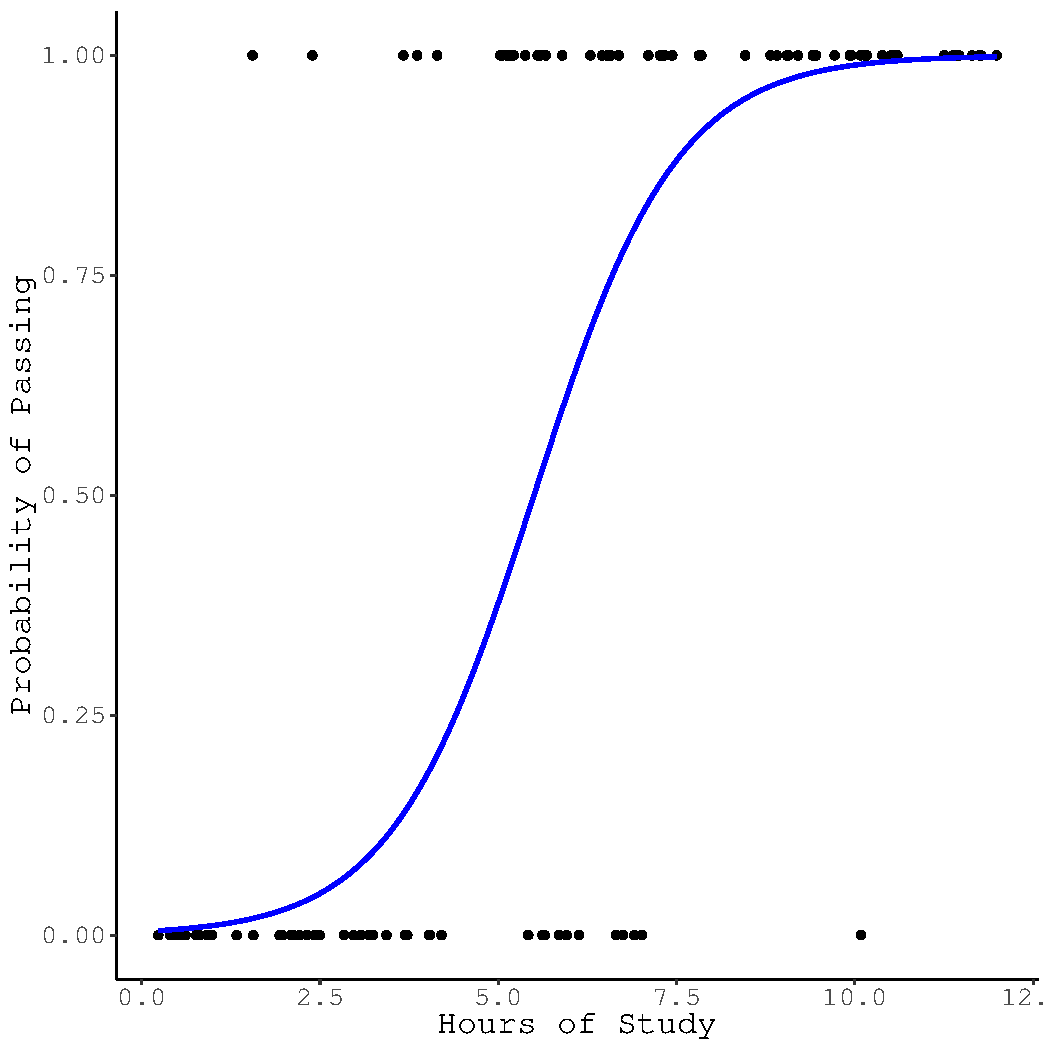
\includegraphics[width=\maxwidth]{figure/unnamed-chunk-3-1} 

}



\end{knitrout}

\end{column}
\end{columns}
  
\end{frame}

\watermarkon %-----------------------------------------------------------------%

\begin{frame}{Defining the Logistic Regression Model}
  
  In logistic regression problems, we are modeling binary data:
  \begin{itemize}
  \item Usual coding: $Y \in \{1 = \text{``Success''}, 0 = \text{``Failure''} \}$.
  \end{itemize}
  \vb
  The \emph{Binomial} distribution is a good way to represent this kind of data.
  \begin{itemize}
  \item The systematic component in our logistic regression model will be the 
    binomial distribution.
  \end{itemize}
  \vb
  The mean of the binomial distribution (with $N = 1$) is the ``success'' 
  probability, $\pi = P(Y = 1)$.
  \begin{itemize}
  \item We are interested in modeling $\mu_Y = \pi$:
    \begin{align*}
      g(\pi) = \beta_0 + \sum_{p = 1}^P \beta_p X_p
    \end{align*}
  \end{itemize}
  
  \comment{%%%%%%%%%%%%%%%%%%%%%%%%%%%%%%%%%%%%%%%%%%%%%%%%%%%%%%%%%%%%%%%%%%%%%% BEGIN \comment{}
  \vc
  \begin{itemize}
  \item The \emph{Bernoulli} distribution is the most natural representation of 
    this type of data.
    \begin{align*}
      \text{Bern}(Y\text{;}~\pi) = \pi^Y(1 - \pi)^{1 - Y}
    \end{align*}
  \item In logistic regression, we work with a generalization of the 
    \emph{Bernoulli} distribution, namely the \emph{Binomial} distribution:
    \begin{align*}
      \text{Bin}(K\text{;}~\pi, N) = \binom{N}{K} \pi^K(1 - \pi)^{N - K}
    \end{align*}
  %\item Note that $Bin(\pi, 1) = Bern(\pi)$.
  \end{itemize}
  }%%%%%%%%%%%%%%%%%%%%%%%%%%%%%%%%%%%%%%%%%%%%%%%%%%%%%%%%%%%%%%%%%%%%%%%%%%%%%% END \comment{}
  
\end{frame}

%------------------------------------------------------------------------------%

\begin{frame}{Link Function for Logistic Regression}
  
  Because $\pi$ is bounded by 0 and 1, we cannot model it directly---we must 
  apply an appropriate link function.
  \vc
  \begin{itemize}
  \item Logistic regression uses the \emph{logit link}.
    \vc
    %\begin{itemize}
  \item Given $\pi$, we can define the \emph{odds} of success as:
    \begin{align*}
      O_s = \frac{\pi}{1 - \pi}
    \end{align*}
  \item Because $\pi \in [0, 1]$, we know that $O_s \geq 0$.
    \vc
  \item We take the natural log of the odds as the last step to fully map 
    $\pi$ to the real line.
    \begin{align*}
      \text{logit}(\pi) = \ln \left(\frac{\pi}{1 - \pi}\right)
    \end{align*}
    %\end{itemize}
  \end{itemize}
  
\end{frame}

%------------------------------------------------------------------------------%

\begin{frame}{Fully Specified Logistic Regression Model}
  
  Our final logistic regression model is:
  \begin{align*}
    Y &\sim \text{Bin}(\pi, 1)\\
    \text{logit}(\pi) &= \beta_0 + \sum_{p = 1}^P \beta_p X_p
  \end{align*}
  The fitted model can be represented as:
  \begin{align*}
    \text{logit}(\hat{\pi}) = \hat{\beta}_0 + \sum_{p = 1}^P \hat{\beta}_p X_p
  \end{align*}
  The fitted coefficients, $\{\hat{\beta}_0, \hat{\beta}_p\}$, are interpreted 
  in units of \emph{log odds}.

\end{frame}

%------------------------------------------------------------------------------%

\begin{frame}{Logistic Regression Example}
  


If we fit a logistic regression model to the test-passing data plotted above, we 
get:
\begin{align*}
  \text{logit}(\hat{\pi}_{pass}) = -3.414 + 0.683 X_{study}
\end{align*}
\vx{-12}
\begin{itemize}
\item A student who does not study at all has -3.414 log odds of passing the
  exam.  
\item For each additional hour of study, a student's log odds of passing increase
  by 0.683 units.
\end{itemize}
\vb
Log odds do not lend themselves to interpretation.
\begin{itemize}
\item We can convert the effects back to an odds scale by exponentiation.
  %\begin{itemize}
\item $\hat{\beta}$ has log odds units, but $e^{\hat{\beta}}$ has odds units.
  %\end{itemize}
\end{itemize}

\end{frame}

%------------------------------------------------------------------------------%

\begin{frame}{Interpretations} 
 
  Exponentiating the coefficients also converts the additive effects to 
  multiplicative effects.
  \vc
  \begin{itemize}
  \item $\ln(AB) = \ln(A) + \ln(B)$
  \item We can interpret $\hat{\beta}$ as we would in linear regression:
    \begin{itemize}
    \item A unit change in $X_p$ produces an expected change of $\hat{\beta}_p$ 
      units in $\text{logit}(\pi)$.
    \end{itemize}
    \vc
  \item After exponentiation, however, unit changes in $X_p$ imply multiplicative 
    changes in $O_s = \pi / (1 - \pi)$.
    \begin{itemize}
    \item A unit change in $X_p$ results in multiplying $O_s$  by 
      $e^{\hat{\beta}_p}$.
    \end{itemize}
  \end{itemize}
  
\end{frame}

%------------------------------------------------------------------------------%

\begin{frame}{Interpretations}
  
  Exponentiating the coefficients in our toy test-passing example produces the 
  following interpretations:
  \begin{itemize}
  \item A student who does not study is expected to pass the exam with odds of 
    0.033.
  \item For each additional hour a student studies, their odds of passing
    increase by 1.98 \emph{times}.
    \begin{itemize}
    \item Odds of passing are \emph{multiplied} by 1.98 for each extra 
      hour of study.
    \end{itemize}
  \end{itemize}
    
  \vb
  \pause
  
  Due to the confusing interpretations of the coefficients, we often focus
  on the valance of the effects: 
  \begin{itemize}
  \item Additional study time is associated with increased odds of passing.
  \item $\hat{\beta_p} > 0$ = ``Increased Success'',  $e^{\hat{\beta}_p} > 1$ = 
    ``Increased Success''
  \end{itemize}
\end{frame}

%------------------------------------------------------------------------------%

\begin{frame}{Multiple Logistic Regression}
  
  The preceding example was a \emph{simple logistic regression}.
  \vc
  \begin{itemize}
  \item Including multiple predictor variables in the systematic component leads 
    to \emph{multiple logistic regression}.
    \vc
  \item The relative differences between simple logistic regression and multiple
    logistic regression are the same as those between simple linear regression
    and multiple linear regression.
    \vc
    \begin{itemize}
    \item The only important complication is that the regression coefficients 
      become partial effects.
    \end{itemize}
  \end{itemize}
  
\end{frame}
  
%------------------------------------------------------------------------------%

\begin{frame}{Multiple Logistic Regression Example}
  


Suppose we want to predict the probability of a patient having ``high'' blood 
glucose from their age, BMI, and average blood pressure.
\vc
\begin{itemize}
\item We could do so with the following model:
  \begin{align*}
    \text{logit}(\pi_{hi.gluc}) = 
    \beta_0 + \beta_1 X_{age.40} + \beta_2 X_{BMI.25} + \beta_3 X_{BP.100}
  \end{align*}
\item By fitting this model to our usual ``diabetes'' data we get:
  \begin{align*}
    \text{logit}(\hat{\pi}_{hi.gluc}) = 
    -1.888 + 0.022 X_{age.40} + 0.126 X_{BMI.25} + 0.027 X_{BP.100}
  \end{align*}
\item Exponentiating the coefficients produces:
  \begin{align*}
    \frac{\hat{\pi}_{hi.gluc}}{1 - \hat{\pi}_{hi.gluc}} = 
    0.151 \times 1.023^{X_{age.40}} \times 1.134^{X_{BMI.25}} \times 
    1.028^{X_{BP.100}}
  \end{align*}
\end{itemize}

\end{frame}

%------------------------------------------------------------------------------%
  
\begin{frame}{Exponentiating the Systematic Component}
  
  \begin{align*}
    \text{logit}(\hat{\pi}_{hi.gluc}) &= -1.888 + 0.022 X_{age.40} + 
    0.126 X_{BMI.25} + 0.027 X_{BP.100}\\[12pt]
    e^{\text{logit}(\hat{\pi}_{hi.gluc})} &= 
    e^{\left(-1.888 ~ + ~ 0.022 X_{age.40} ~ + ~ 0.126 X_{BMI.25} 
      ~ + ~ 0.027 X_{BP.100} \right)}\\[8pt]
    \frac{\hat{\pi}_{hi.gluc}}{1 - \hat{\pi}_{hi.gluc}} &= 
    e^{-1.888} \times e^{0.022 X_{age.40}} \times e^{0.126 X_{BMI.25}} \times 
    e^{0.027 X_{BP.100}}\\[8pt]
    &= \left(e^{-1.888}\right) \times \left(e^{0.022}\right)^{X_{age.40}} \times 
    \left(e^{0.126}\right)^{X_{BMI.25}} \times 
    \left(e^{0.027}\right)^{X_{BP.100}}\\[14pt]
    &= 0.151 \times 1.023^{X_{age.40}} \times 1.134^{X_{BMI.25}} 
    \times 1.028^{X_{BP.100}}
  \end{align*}

\end{frame}

%------------------------------------------------------------------------------%

\begin{frame}{}
  
  \begin{center}
    \Huge{\textsc{Multinomial Logistic Regression}}
  \end{center}
  
\end{frame}

%------------------------------------------------------------------------------%

\begin{frame}{Multi-Class Outcomes}
  
  So, what do we do if our outcome takes more than two levels?
  \begin{itemize}
    \item Voting intention = \{Will vote, Won't vote, Not sure\}
    \item Preferred caffeine source = \{Coffee, Tea, Energy drink, None\}
    \item Current mood = \{Happy, Sad, Angry, Neutral\}
  \end{itemize}
  \vb
  \pause
  We saw that using a nominal variable with $L$ response levels as a predictor 
  requires creating $L - 1$ dummy codes.
  \begin{itemize}
  \item We could solve our problem by estimating $L - 1$ separate logistic 
    regression models.
  \item Do you see any problems with that approach?
  \end{itemize}
  \vb
  \pause
  We have a better way: \emph{Multinomial logistic regression}.
  
\end{frame}

%------------------------------------------------------------------------------%

\begin{frame}{Defining the Multinomial Logistic Regression Model}
  
  In multinomial logistic regression problems, we are modeling multi-class 
  nominal data:
  \begin{itemize}
  \item Usual coding: $Y \in \{1, 2, \ldots, L\}$.
  \end{itemize}
  \vb
  The \emph{Multinomial} distribution---a generalization of the binomial 
  distribution---is a good way to represent this kind of data.
  \begin{itemize}
  \item The systematic component in our multinomial logistic regression model 
    will be the multinomial distribution.
  \end{itemize}
  \vb
  We are interested in modeling the $L - 1$ probabilities, $\pi_l = P(Y = l)$, 
  of endorsing each response level instead of the \emph{baseline} level.
  \begin{align*}
    g(\pi_l) = \beta_{l0} + \sum_{p = 1}^P \beta_{lp} X_p, ~~ l = 2, 3, \ldots, L
  \end{align*}

\end{frame}

%------------------------------------------------------------------------------%

\begin{frame}{Full Multinomial Logistic Regression Model}
  
  Given $L$ unique response levels for $Y$, our final multinomial logistic 
  regression model is:
  \begin{align*}
    Y &\sim \text{Multinom}(\Pi, \mathbf{1}), ~~ \Pi = \{\pi_2, \pi_3, \ldots, 
    \pi_L\}\\
    \text{logit}(\pi_l) &= \beta_{l0} + \sum_{p = 1}^P \beta_{lp} X_p, ~~ l = 2, 3,
    \ldots, L
  \end{align*}
  The fitted model can be represented as:
  \begin{align*}
    \text{logit}(\hat{\pi}_l) = \hat{\beta}_{l0} + \sum_{p = 1}^P \hat{\beta}_{lp} 
    X_p, ~~ l = 2, 3, \ldots, L
  \end{align*}
  Note that we, \emph{simultaneously}, estimate $L - 1$ separate sets of 
  coefficients, $\{\beta_{l0}, \beta_{lp}\}$.   
  
\end{frame}

%------------------------------------------------------------------------------%

\begin{frame}[allowframebreaks, fragile]{Example}



Suppose we want to predict the probability of a patient having ``high'' or 
``moderate'' blood glucose, versus ``low'' blood glucose, from their age, BMI, 
and average blood pressure.
\vc
\begin{itemize}
\item We could do so with the following model:
  \begin{align*}
    \text{logit}(\pi_l) = 
    \beta_{l0} + \beta_{l1} X_{age.40} + \beta_{l2} X_{BMI.25} + \beta_{l3} X_{BP.100}
  \end{align*}
\item By fitting this model to our usual ``diabetes'' data we get:
  \begin{align*}
    \text{logit}(\hat{\pi}_{hi.gluc}) &= 
    -0.022 + 0.035 X_{age.40} + 0.241 X_{BMI.25} + 
    0.067 X_{BP.100}\\[8pt]
    \text{logit}(\hat{\pi}_{mid.gluc}) &= 
    1.626 + 0.016 X_{age.40} + 0.132 X_{BMI.25} + 
    0.046 X_{BP.100}
  \end{align*}
\end{itemize}

\pagebreak

\begin{itemize}
\item Exponentiating the coefficients produces:
  \begin{align*}
    \frac{\hat{\pi}_{hi.gluc}}{\hat{\pi}_{low.gluc}} &= 
    0.978 \times 1.036^{X_{age.40}} \times 1.272^{X_{BMI.25}} 
    \times 1.07^{X_{BP.100}}\\[8pt]
    \frac{\hat{\pi}_{mid.gluc}}{\hat{\pi}_{low.gluc}} &= 
    5.084 \times 1.016^{X_{age.40}} \times 1.141^{X_{BMI.25}} 
    \times 1.047^{X_{BP.100}}
  \end{align*}
\end{itemize}

\end{frame}

%------------------------------------------------------------------------------%
  
\begin{frame}{}
  
  \begin{center}
    \Huge{\textsc{Classification}}
  \end{center}
  
\end{frame}

%------------------------------------------------------------------------------%

\begin{frame}{Predictions from Logistic Regression}
  
  Given a fitted logistic regression model, we can get predictions for new 
  observations of $\{X_p\}$, $\{X_p'\}$.
  \vc
  \begin{itemize}
  \item Directly applying $\{\hat{\beta}_0, \hat{\beta}_p\}$ to $\{X_p'\}$ will 
    produce predictions on the scale of $\eta$:
    \begin{align*}
      \hat{\eta}' = \hat{\beta}_0 + \sum_{p = 1}^P \hat{\beta}_p X_p'
    \end{align*}
  \item By applying the inverse link function, $g^{-1}(\cdot)$, to
    $\hat{\eta}'$, we get predicted success probabilities:
    \begin{align*}
      \hat{\pi}' = g^{-1}(\hat{\eta}')
    \end{align*}
  \end{itemize}
  
\end{frame}

%------------------------------------------------------------------------------%

\begin{frame}{Predictions from Logistic Regression}
  
  In logistic regression, the inverse link function, $g^{-1}(\cdot)$, is the
  \emph{logistic function}:
  \begin{align*}
    \text{logistic}(X) = \frac{e^X}{1 + e^X}
  \end{align*}
  So, we convert $\hat{\eta}'$ to $\hat{\pi}'$ by:
  \begin{align*}
    \hat{\pi}' &= \frac{e^{\hat{\eta}'}}{1 + e^{\hat{\eta}'}} = \frac{\exp \left( 
      \hat{\beta}_0 + \sum_{p = 1}^P \hat{\beta}_p X_p' \right) }{1 + \exp \left( 
      \hat{\beta}_0 + \sum_{p = 1}^P \hat{\beta}_p X_p' \right) }
  \end{align*}
  
\end{frame}

%------------------------------------------------------------------------------%

\begin{frame}{Classification with Logistic Regression}
  
  Once we have computed the predicted success probabilities, $\hat{\pi}'$, we 
  can use them to classify new observations.
  \vc
  \begin{itemize}
  \item By choosing a threshold on $\hat{\pi}'$, say $\hat{\pi}' = t$, we can 
    classify the new observations as ``Successes'' or ``Failures'':
    \begin{align*}
      \hat{Y}' = \left\{ 
      \begin{array}{ccc}
        1 & if & \hat{\pi}' \geq t\\
        0 & if & \hat{\pi}' < t\\
      \end{array}
      \right.
    \end{align*}
    
  \end{itemize}
  
\end{frame}

%------------------------------------------------------------------------------%

\begin{frame}[allowframebreaks]{Classification Example}
  


Say we want to classify a new patient into either the ``high glucose'' group 
or the ``not high glucose'' group using the model fit above.
\begin{itemize}
\item Assume this patient has the following characteristics:
  \begin{itemize}
  \item They are 57 years old
  \item Their BMI is 28
  \item Their average blood pressure is 92
  \end{itemize}
\end{itemize}
\vb
First we plug their predictor data into the fitted model to get their 
model-implied $\eta$:
\begin{align*}
  \hat{\eta} &= -1.888 + 0.022 (57 - 40) + 0.126 (28 - 25) + 0.027 (92 - 100)\\
  &= -1.347 
\end{align*}

\pagebreak

Next we convert the predicted $\eta$ value into a model-implied success
probability by applying the logistic function:
\begin{align*}
  0.206 = \frac{e^{-1.347}}{1 + e^{-1.347}}
\end{align*}\\
\vb
Finally, to make the classification, assume a threshold of $\hat{\pi}' = 0.5$ as 
the decision boundary.
\begin{itemize}
\item Because $0.206 < 0.5$ we would classify this 
  patient into the ``low glucose'' group.
\end{itemize}

\end{frame}
   
%------------------------------------------------------------------------------%

\begin{frame}{Predictions from Multinomial Logistic Regression}
  
  Generating predictions from a multinomial logistic regression model is nearly 
  identical to predicting with a logistic regression model.
  \vc
  \begin{itemize}
  \item The only difference is that the multinomial logistic regression model 
    will produce $L$ distinct estimates of $\hat{\eta}_l'$ and $\hat{\pi}_l'$:
    \begin{align*}
      \hat{\eta}_l' &= 
      \begin{cases}
        \hat{\beta}_{l0} + \sum_{p = 1}^P \hat{\beta}_{lp} X_p' & \text{if $l > 1$}\\
        0 & \text{if $l = 1$}
      \end{cases}\\[8pt]
      \hat{\pi}_l' &= g^{-1}(\hat{\eta}_l')
    \end{align*}
  \end{itemize}
  
  %\item The success probability for the baseline level, $\hat{\pi}_1$, is defined 
  %  by the other $L - 1$ $\hat{\pi}_l$ values:
  %  \begin{align*}
  %    \hat{\pi}_1 = 1 - \sum_{l = 2}^L\hat{\pi}_l
  %  \end{align*}
  %\end{itemize}
\end{frame}

%------------------------------------------------------------------------------%

\begin{frame}{Predictions from Multinomial Logistic Regression}
  
  In multinomial logistic regression, the inverse link function, $g^{-1}(\cdot)$, 
  is the \emph{softmax function}:
  \begin{align*}
    \text{softmax}(X_l) = \frac{e^{X_l}}{\sum_{j = 1}^Je^{X_j}}
  \end{align*}
  So, we convert each $\hat{\eta}_l'$ to $\hat{\pi}_l'$ by:
  \begin{align*}
    \hat{\pi}_l' = \frac{e^{\hat{\eta}_l'}}{\sum_{j = 1}^J e^{\hat{\eta}_j'}} = 
    \begin{cases}
      \frac{\exp \left( 
        \hat{\beta}_{l0} + \sum_{p = 1}^P \hat{\beta}_{lp} X_p' \right) }
           {1 + \sum_{j = 2}^J \exp \left(
             \hat{\beta}_{j0} + \sum_{p = 1}^P \hat{\beta}_{jp} X_p' 
             \right) } & \text{if $l > 1$}\\[16pt]
           \frac{1}
                {1 + \sum_{j = 2}^J \exp \left(
                  \hat{\beta}_{j0} + \sum_{p = 1}^P \hat{\beta}_{jp} X_p' 
                  \right) } & \text{if $l = 1$}
    \end{cases}
  \end{align*}
           
\end{frame}

%------------------------------------------------------------------------------%

\begin{frame}{Classification with Multinomial Logistic Regression}
  
  Once we have computed the $L$ predicted success probabilities, $\hat{\pi}_l'$, 
  we can use them to classify new observations.
  \vc
  \begin{itemize}
  \item Each observation is labeled with the response level associated with the 
    largest $\hat{\pi}_l'$
    \vc
  \item For example:
    \begin{itemize}
    \item Given the response options $Y \in $
      \{Coffee, Tea, Energy Drinks, None\}
      \vc
    \item And corresponding success probabilities $\hat{\pi}_l \in 
      \{0.45, 0.2, 0.15, 0.2\}$
      \vc
    \item We would assign the observation to the ``Coffee'' group 
    \end{itemize}
  \end{itemize}

\end{frame}

%------------------------------------------------------------------------------%

\begin{frame}[fragile, allowframebreaks]{Classification Example}
  


Let's re-classify our patient into either the ``high glucose'', ``moderate 
glucose'', or ``low glucose'' group using the model fit above.
\begin{itemize}
\item First we plug their predictor data into the fitted model to get their 
  set of model-implied $\eta_l$ values:
\end{itemize}
%\begin{align*}
%  \text{logit}\left(\frac{\pi_{low.gluc}}{\pi_{low.gluc}}\right) &= 
%  b10 &+ b11 (57 - 40) &+ b12 (28 - 25)\\ &+ b13 (92 - 100) &= 
%  eta2[1]\\
%  \text{logit}\left(\frac{\pi_{mid.gluc}}{\pi_{low.gluc}}\right) &=
%  b20 &+ b21 (57 - 40) &+ b22 (28 - 25)\\ &+ b23 (92 - 100) &=
%  eta2[2]\\
%  \text{logit}\left(\frac{\pi_{hi.gluc}}{\pi_{low.gluc}}\right) &=
%  b30 &+ b31 (57 - 40) &+ b32 (28 - 25)\\ &+ b33 (92 - 100) &=
%  eta2[3]
%\end{align*}
%\end{itemize}

\vc

\setlength\tabcolsep{1.5pt} % decrease column padding in tabular

\begin{tabular}{rllll}
  $\text{logit}\left(\frac{\pi_{low.gluc}}{\pi_{low.gluc}}\right)$ &=&&&\\ 
  0 &+ 0 (57 - 40) &+ 0 (28 - 25) &+ 0 (92 - 100) &= 
  0\\[8pt]
  $\text{logit}\left(\frac{\pi_{mid.gluc}}{\pi_{low.gluc}}\right)$ &=&&&\\
  1.626 &+ 0.016 (57 - 40) &+ 0.132 (28 - 25) &+ 0.046 (92 - 100) &=
  1.929\\[8pt]
  $\text{logit}\left(\frac{\pi_{hi.gluc}}{\pi_{low.gluc}}\right)$ &=&&&\\
  -0.022 &+ 0.035 (57 - 40) &+ 0.241 (28 - 25) &+ 0.067 (92 - 100) &=
  0.762
\end{tabular}

\setlength\tabcolsep{6pt} % back to the default value

\pagebreak

\begin{itemize}
\item Next we apply the softmax function to convert the predicted $\eta_l$ 
  values into model-implied success probabilities:
\end{itemize}
\begin{align*}
  \hat{\pi}_{low.gluc} &=  
  \frac{1}{1 + e^{1.929} + e^{0.762}} = 
  0.1\\[8pt]
  \hat{\pi}_{mid.gluc} &= 
  \frac{e^{1.929}}{1 + e^{1.929} + e^{0.762}} = 
  0.687\\[8pt]
  \hat{\pi}_{hi.gluc} &= 
  \frac{e^{0.762}}{1 + e^{1.929} + e^{0.762}} =
  0.214  
\end{align*}
\begin{itemize}
\item Finally, to make the classification, we find the largest $\hat{\pi}_l'$:
  \begin{itemize}
  \item Because $\hat{\pi}_{mid.gluc} = 0.687$ is the 
    largest, we would classify this patient into the 
    ``moderate glucose'' group.
  \end{itemize}
\end{itemize}

\end{frame}

%------------------------------------------------------------------------------%

\begin{frame}{Classification Error}
  
  The MSE is not an appropriate error measure for classification.
  \begin{itemize}
  \item The differences between predicted and observed outcomes have little
    meaning.
  \end{itemize}
  \vb
  One of the most popular error measures is the \emph{Cross-Entropy Error}:
  \begin{align*}
    CEE &= -N^{-1} \sum_{n = 1}^N Y_n \ln(\hat{\pi}_n) + (1 - Y_n)\ln(1 - \hat{\pi}_n)\\
    CEE &= -N^{-1} \sum_{n = 1}^N \sum_{l = 1}^L \textbf{I}(Y_n = l) \ln(\hat{\pi}_{nl})
  \end{align*}
  \vx{-6}
  \begin{itemize}
  \item The CEE is sensitive to classification confidence.
  \item Stronger predictions are more heavily weighted.
  \end{itemize}
  
\end{frame}

%------------------------------------------------------------------------------%

\begin{frame}{Why not Missclassification Rate?}
  


 The missclassification rate is a na\"{i}vely appealing option.
  \begin{itemize}
  \item The proportion of cases assigned to the wrong group
  \end{itemize}
  \vb
  Consider two perfect classifiers:
  \begin{enumerate}
  \item $P(\hat{Y}_n = 1 | Y_n = 1) = 0.90$,  $P(\hat{Y}_n = 1 | Y_n = 0) = 0.10$, $n = 1, 2, \ldots, N$
  \item $P(\hat{Y}_n = 1 | Y_n = 1) = 0.55$,  $P(\hat{Y}_n = 1 | Y_n = 0) = 0.45$, $n = 1, 2, \ldots, N$
  \end{enumerate}
  \vb
  Both of these classifiers will have the same missclassification rate.
  \begin{itemize}
  \item Neither model ever makes an incorrect group assignment.
  \end{itemize}
  \vb
  The first model will have a lower CEE.
  \begin{itemize}
  \item The classifications are made with higher confidence.
  \item $CEE_1 = 0.105$, $CEE_2 = 0.598$
  \end{itemize}
  
\end{frame}

%------------------------------------------------------------------------------%

\begin{frame}{Conclusion}
  
  \begin{itemize}
  \item The Generalized Linear Model is a flexible class of models that we can
    use for non-normally distributed outcomes.
    \begin{itemize}
    \item Multiple linear regression is a special type of GLM.
    \end{itemize}
    \vc
  \item We cannot model nominal outcomes with linear regression.
    \begin{itemize}
    \item We should use some form of logistic regression.
    \end{itemize}
    \vc
  \item We use logistic regression for binary outcomes and multinomial logistic
    regression for multi-class nominal outcomes.
    \vc
  \item We must take care when interpreting the coefficients from logistic
    regression models.
    \vc
  \item We can use the estimated success probabilities from a fitted model to
    classify new observations.
  \end{itemize}
  
\end{frame}

%------------------------------------------------------------------------------%

\end{document}

